\section{Nonlinear frequency limits at fixed measurement buses}
\label{sec:nonlinear-fixed-bus}

\paragraph{Question and contribution boundary.}
Can redistributing a fixed amount of inertia, or adding damping that only
redistributes power, remove every local frequency overshoot? We answer a
precise version for a nonlinear lossless swing network with causal primary
response. The answer follows from two equilibria, rather than a linearized
transient. We obtain a necessary total-inertia bound for arbitrary fixed
events, a graph-resistance expression for a localized event, and a sharp
two-node example with a constructive controller above the bound.
These results do not identify an optimal SG--GFL replacement in the detailed
IEEE--39 model. Inertia allocation, graph performance metrics and integral
response restrictions have substantial prior work
\cite{poollainertia,pagnier,malladamoments,aalipourmoments}.
Aggregate-neutral damping is also a direct recent antecedent
\cite{kohlhaas2026}. The specific candidate contribution is the finite
endpoint constraint and its quantified exclusion of a controller class.
The distinction between a well-shaped COI response and local oscillations
is already established, including recent frequency-shaping design
\cite{jiangfs}; the sharp finite-amplitude obstruction below is the result
to compare, rather than that general distinction.

\subsection{Physical class, fixed events and fixed outputs}
Use scaled electrical angle $q=\theta/\omega_b$ and per-unit frequency
deviation $\nu=\dot q$. Consider
\begin{equation}
 M\dot\nu+(h*\nu)(t)+F(q)=p^0+d\,1_{t\geq0}+u(t),\qquad
 F(q)=B\diag(\gamma_e)\sin(\omega_bB^Tq).
 \label{eq:nfl-model}
\end{equation}
Here $M\succ0$ is diagonal, the graph is connected, $\gamma_e>0$, and
voltage magnitudes are fixed. In particular $\one^TF(q)=0$.
The causal matrix-valued kernel $h$ may contain instantaneous and delayed
atoms; assume finite total variation and first moment. Write
\[
 \mathcal D(s)=D_0+sD_1+o(s),\quad
 m=\one^TM\one,\quad d_0=\one^TD_0\one>0,\quad
 \kappa=\one^TD_1\one,\quad c_D=D_0^T\one/d_0.
\]
No derivative-of-delta inertial feedthrough is hidden in $h$.
Such a realization requires an explicit, justified change of $M$.
Initially $F(q^0)=p^0$ and $\nu(t)=0$ for $t\leq0$.
Let $P=\one^Td\ne0$, $u(t)\to0$, and
$Q=\int_0^\infty\one^Tu(t)\,dt$ be finite.
Every trajectory to which the theorem is applied must converge with
integrable transients to
\[
 \nu\to\Omega\one,\qquad q-q^0-\Omega t\one\to\eta_\infty,
 \qquad \Omega=P/d_0.
\]
Existence of an endpoint is not a proof of convergence.
The final relative shape $\delta$ equals $\eta_\infty$ modulo a common
rotation and solves
\begin{equation}
 F(q^0+\delta)-F(q^0)=d-(P/d_0)D_0\one.
 \label{eq:nfl-endpoint}
\end{equation}
For fixed network, $D_0,d$ and equilibrium branch, this equation is
independent of the distribution and total amount of $M$.
Actual removal of SG generally changes more than $M$ and need not preserve
this contract.

\begin{theorem}[Finite endpoint law for a fixed output]
For a fixed vector $a$ satisfying $a^T\one=1$, define
$A_a=\int_0^\infty(\Omega-a^T\nu(t))\,dt$. Under the preceding assumptions,
\begin{equation}
 \boxed{A_a=\frac{P(m+\kappa)}{d_0^2}
              +(c_D-a)^T\delta-\frac{Q}{d_0}.}
 \label{eq:nfl-fixed-area}
\end{equation}
\end{theorem}
\status{EXACT\_IDENTITY}
\begin{proof}
Integration of the summed balance, after subtracting its final value, gives
\[
 (m+\kappa)\Omega+\one^TD_0\eta_\infty=Q.
\]
The memory contribution follows from
$\int_0^\infty[(h*\nu)-D_0\Omega\one]\,dt
=D_0\eta_\infty+\Omega D_1\one$.
This is Fubini's identity for a kernel with the stated moments.
Since $A_a=-a^T\eta_\infty$ and
$(c_D-a)^T\one=0$, eliminating the common rotation proves the result.
\end{proof}

Consequently, keeping $m,D_0,D_1,d,\delta,Q$ fixed preserves the area of
\emph{every fixed measurement bus}, even if inertia is redistributed and
the control law changes. Also
$A_i-A_j=\delta_j-\delta_i$.
The trajectories, peaks, modal damping and settling times need not be
invariant. An optimization of COI area must be interpreted carefully:
its output weights $a=M\one/m$ themselves change with inertia allocation.
An improved COI area can therefore reflect reweighting of unchanged nodal
areas. The fixed-output theorem avoids that ambiguity.

\subsection{A necessary all-bus bound and its graph form}
Absence of crossing beyond the final frequency means
$\operatorname{sign}(P)(\nu_j(t)-\Omega)\leq0$ for every monitored bus and
every $t\geq0$. Continuity from $\nu_j(0)=0$ makes $A_j/P>0$ necessary,
strictly. For a finite family of fixed events, put
$v_e=\delta_e/P_e$ and
$\Phi_e=\max_{j\in\mathcal O}(v_{e,j}-c_D^Tv_e)$.
Equation~\eqref{eq:nfl-fixed-area} implies
\begin{equation}
 \boxed{m>\max_e\left\{-\kappa+d_0^2\Phi_e+
                              d_0 Q_e/P_e\right\}.}
 \label{eq:nfl-general-floor}
\end{equation}
The weak inequality is only the closure of a necessary condition.
Neither version guarantees convergence or absence of overshoot.
The event $d_e$ is fixed when comparing inertia assignments; it is not
silently redistributed in proportion to the new $M$.

Assume now $D_0$ is positive diagonal, $c=D_0\one/d_0$, and the initial
and final shapes lie in one cohesive angle cell. Define the exact secant
operator
\begin{align}
 \bar L_e&=\int_0^1J_F(q^0+t\delta_e)\,dt
          =B\diag(\bar w_{\ell,e})B^T,\\
 \bar w_{\ell,e}
    &=\omega_b\gamma_\ell\int_0^1
          \cos\!\left(\omega_b B_\ell^T(q^0+t\delta_e)\right)\,dt>0.
 \label{eq:nfl-secant}
\end{align}
It is a genuine Laplacian on this domain. No initial-Jacobian substitution
has been made.

\begin{theorem}[Localized event and a placement-independent floor]
For $d=P e_k$, with every bus monitored, define
\begin{equation}
 \mathcal R_k(P)=(e_k-c)^T\bar L_k^\dagger(e_k-c).
 \label{eq:nfl-resistance}
\end{equation}
Then $\Phi=\mathcal R_k(P)$ and the most restrictive nodal \emph{area}
constraint is at the disturbed bus $k$. With $Q=0$,
\begin{equation}
 \boxed{m+\kappa>d_0^2\mathcal R_k(P)}
 \label{eq:nfl-local-floor}
\end{equation}
is necessary for absence of local final-frequency crossing, for every
inertia distribution and every convergent energy-neutral supplementary
controller preserving the same endpoint.
\end{theorem}
\status{PROVED\_REDUCED\_MODEL}
\begin{proof}
The endpoint equation gives $\bar L_kv=e_k-c$.
Set $\phi=v-\one c^Tv$ so that $c^T\phi=0$.
At any maximum with index $j\ne k$,
$(\bar L_k\phi)_j=\sum_l\bar w_{jl}(\phi_j-\phi_l)\geq0$,
contradicting $(e_k-c)_j=-c_j<0$.
Thus the maximum is at $k$, and
$\phi_k=(e_k-c)^T\bar L_k^\dagger(e_k-c)$.
Substitution in \eqref{eq:nfl-general-floor} proves the bound.
\end{proof}
This does not identify the bus of the largest instantaneous frequency peak.
For nonnegative damping with some zero entries, the maximum is still
attained at $k$, but uniqueness needs qualification.

The graph quantity has the exact representations
\begin{equation}
 \mathcal R_k(P)=
 \sum_{\ell>0}\frac{|u_\ell^T(e_k-c)|^2}{\lambda_\ell}
 =\min_{Bf=e_k-c}\sum_\ell\frac{f_\ell^2}{\bar w_{\ell,k}}.
 \label{eq:nfl-gsp-flow}
\end{equation}
These are classical spectral and Thomson identities applied to the
finite secant graph. For every cut $C$ containing $k$,
\begin{equation}
 \mathcal R_k(P)\geq
 \frac{[1-c(C)]^2}{\sum_{\ell\in\partial C}\bar w_{\ell,k}}
 \geq\frac{[1-c(C)]^2}
                {\omega_b\sum_{\ell\in\partial C}\gamma_\ell}.
 \label{eq:nfl-cut}
\end{equation}
Indeed the net unit flow through the cut is $1-c(C)$; weighted
Cauchy--Schwarz gives the first inequality, and $\bar w\leq\omega_b\gamma$
the second. A weak cut separating the event from primary response creates
a calculable necessary support requirement. Strengthening a physical line
also moves the endpoint; these formulas do not prove a frozen-endpoint
monotonic improvement of actual nadir.

\subsection{Latency, measurement windows and energy}
For delayed frequency damping
$\mathcal D(s)=\diag(d_i e^{-s\tau_i})$,
$\kappa=-\sum_i d_i\tau_i$. The delays are fixed physical parameters.
This is not the same channel as a delayed PLL detector.
A causal rectangular measurement
$\nu_{j,W}(t)=[q_j(t)-q_j(t-W)]/W$ satisfies
\begin{equation}
 A_{j,W}=A_j+\Omega W/2.
 \label{eq:nfl-window}
\end{equation}
This follows by integrating the difference between a signal and its
causal average; equivalently its filter has first moment $W/2$.
Therefore the necessary measured-frequency bound is
\begin{equation}
 \boxed{m>\sum_i d_i\tau_i+d_0^2\mathcal R_k(P)
                        +d_0Q/P-d_0W/2.}
 \label{eq:nfl-delay-window}
\end{equation}
A measurement window can make this area-based obstruction vacuous.
The term $d_0W/2$ is not physical inertia. Strictness here assumes
continuous angle/frequency from rest; algebraic phase jumps require their
actual filtered-output contract.

Let $E_{\rm op}=-\operatorname{sign}(P)Q$ be net energy opposing the
disturbance. The unfiltered localized bound becomes
\begin{equation}
 \boxed{E_{\rm op}>
     \frac{|P|}{d_0}\left[d_0^2\mathcal R_k(P)-m-\kappa\right]}
 \label{eq:nfl-energy}
\end{equation}
when the right side is positive. This is net energy over the declared
horizon, not rated battery capacity, and is necessary rather than sufficient.
A storage device that later recharges to $Q=0$ may move a required crossing
to a late, small excursion. A regulatory frequency limit does not generally
require zero crossing of the final value.

For finite $T$, define
$A_{j,T}=\int_0^T(\Omega-\nu_j)\,dt$,
$Q_T=\int_0^T\one^Tu\,dt$ and
\[
 R_h(T)=\int h(dv)\int_{\max(0,T-v)}^T\nu(a)\,da,\qquad
 \delta_T=q(T)-q^0\quad\text{modulo rotation}.
\]
The exact lossless identity is
\begin{equation}
 d_0A_{j,T}=m\nu_{\rm COI}(T)-\one^TR_h(T)
                   +d_0(c_D-e_j)^T\delta_T-Q_T.
 \label{eq:nfl-finite}
\end{equation}
Suppose the first three terms on the right are enclosed within
$\varepsilon_{j,T}$ of
$(m+\kappa)\Omega+d_0(c_D-e_j)^T\delta$.
Then absence of crossing at $j$ up to $T$ requires
$E_{{\rm op},T}>-d_0\operatorname{sign}(P)A_{j,0}
 -\varepsilon_{j,T}$, where $A_{j,0}$ denotes the infinite-horizon
zero-energy endpoint value. Such an enclosure must include terminal shape,
frequency and the entire memory integral, including a bounded tail for
kernels of infinite support. No such IEEE--39 enclosure
has been certified here.

\subsection{A sharp two-node limit with an explicit control}
\begin{theorem}[Sharp inertia infimum in a nonlinear two-node class]
In dimensionless units, let $\mathcal D(s)\equiv I_2$ (instantaneous damping,
no memory), and $F=(\sin z,-\sin z)$ with
$z=q_1-q_2$, $q^0=\nu^0=0$, and $d=(P,0)$, $0<P<2$.
Let admissible controllers satisfy $u_2=-u_1$, $u(t)\to0$,
continuous state velocities and convergence to
$z_*=\arcsin(P/2)$, $\Omega=P/2$.
Across all positive inertia allocations of total $m$ and all such
controllers, the infimum total inertia admitting
$|\nu_j(t)|\leq\Omega$ for both buses and all time is
\begin{equation}
 \boxed{m_{\inf}(P)=\frac{2\arcsin(P/2)}{P}.}
 \label{eq:nfl-sharp}
\end{equation}
The infimum is not attained. The claim imposes no actuator, communication
or control-gain limit.
\end{theorem}
\status{PROVED\_REDUCED\_MODEL}
\begin{proof}
Here $c=(1/2,1/2)^T$ and
$d_0^2\mathcal R_1(P)=2z_*/P$, so necessity for any allocation follows
from \eqref{eq:nfl-local-floor}; equality also forces a crossing.
For sufficiency choose $M=(m/2)I_2$ and $m>2z_*/P$.
Put $k=2/m$, choose
\[
 \ell>\frac{z_*k^2}{P-z_*k},\qquad
 a=z_*\,\frac{k(k+\ell)}{\ell}<P,
\]
and prescribe
\begin{align}
 w(t)&=\Omega(1-e^{-kt}),\\
 z(t)&=a\left[\frac{1-e^{-kt}}{k}
                    -\frac{1-e^{-(k+\ell)t}}{k+\ell}\right],\\
 u_1(t)&=\frac m4\ddot z+\frac12\dot z+\sin z-\frac P2,\qquad
 u_2(t)=-u_1(t). \label{eq:nfl-construction}
\end{align}
Take $\nu_1=w+\dot z/2$, $\nu_2=w-\dot z/2$.
Their sum obeys $m\dot w+2w=P$ and their difference obeys
$(m/2)\ddot z+\dot z+2\sin z=P+2u_1$, proving both original equations.
The initial state is continuous and at rest.
Since $0\leq\dot z=a e^{-kt}(1-e^{-\ell t})<P e^{-kt}$,
both $\nu_j\leq\Omega$, while $\nu_1\geq0$ and $\nu_2\geq-\Omega$.
Also $z\to z_*$ monotonically inside the cohesive interval and $u\to0$.
The control is bounded for each fixed $m>m_{\inf}$ and has zero aggregate
power at all times. This supplies an admissible construction for every
strictly larger $m$.
\end{proof}
The construction can require arbitrarily large power as $m\downarrow
m_{\inf}$. It proves no sharp threshold with physical actuator limits.
Bus 2 can transiently move opposite to the event, although its absolute
frequency deviation remains within $\Omega$.

\paragraph{Monotone COI does not remove the obstruction.}
Set $P=1$ and $m=41/40<\pi/3$ with equal inertia allocation.
For any aggregate-balanced control, $w(t)=\tfrac12(1-e^{-2t/m})$ is
monotone, yet
\[
 A_1=\frac{123-40\pi}{480}<0,\qquad
 A_{\rm COI}=\frac{41}{160}>0.
\]
The uncontrolled trajectory converges: in the rotating frame use
$V=\tfrac12(\nu-\Omega\one)^TM(\nu-\Omega\one)
 +1-\cos z-z/2$.
Then $\dot V=-(\nu-\Omega\one)^T(\nu-\Omega\one)$ and
$V(0)=41/320<1-\pi/4$, the smaller potential at $z=\pm\pi/2$.
The trajectory stays cohesive, and LaSalle on the rotational quotient
gives the unique synchronized endpoint. Thus the forbidden local crossing
is not inferred from an unstable or nonexistent endpoint.
The initial-Jacobian threshold is only $1$ and misses this finite-amplitude
case. The area test is a necessary test; a positive linearized area never
constituted a proof of no crossing.

\begin{figure}[htbp]
\centering
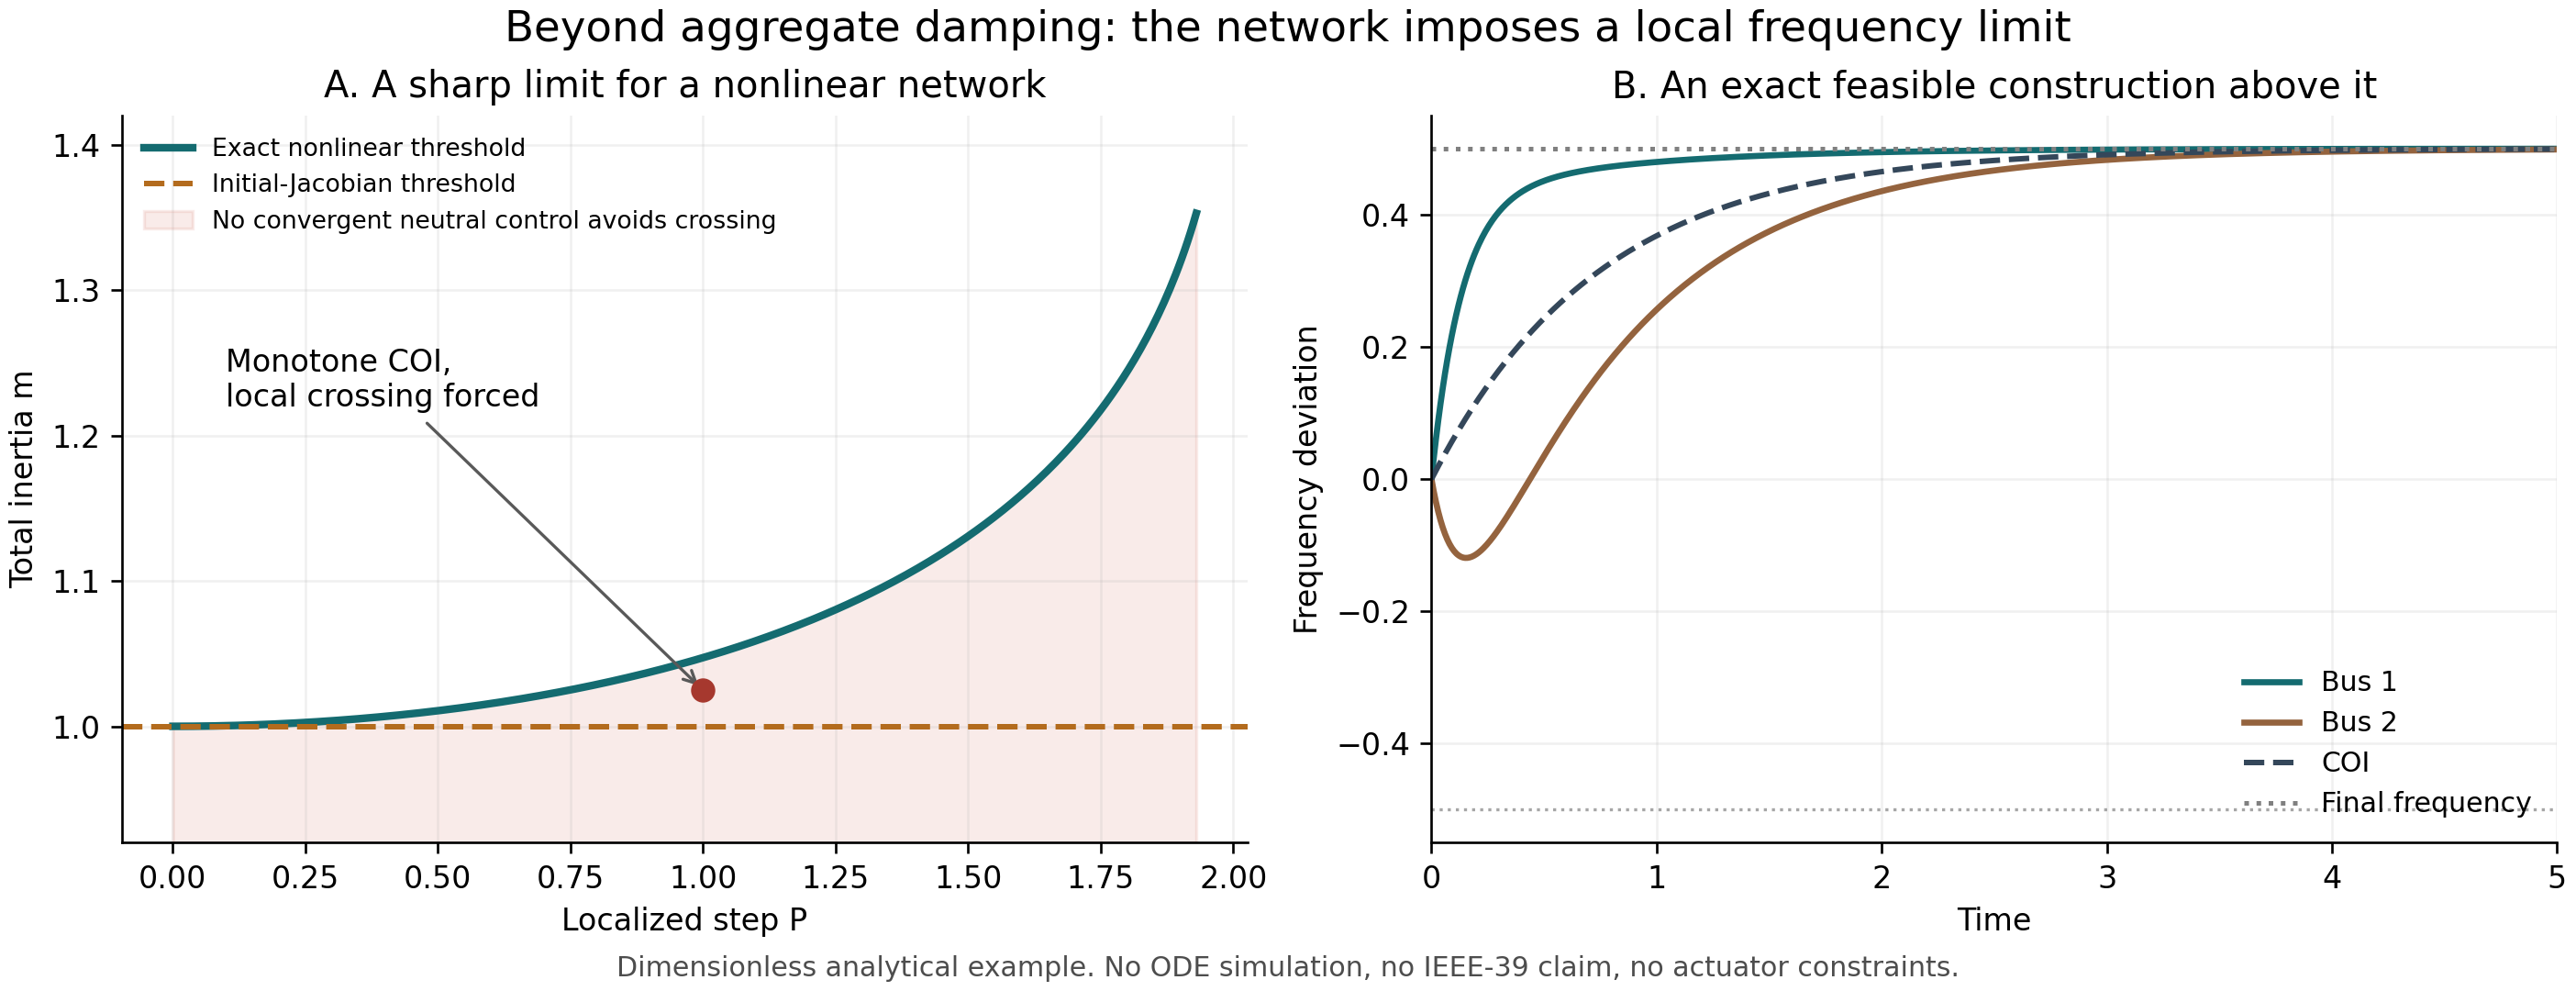
\includegraphics[width=\linewidth]{experiments/nonlinear_frequency_limits_20261004/FIG_SHARP_NETWORK_LIMIT.png}
\caption{Exact dimensionless construction, not an ODE simulation.
Left: the finite-amplitude threshold and its initial-Jacobian counterpart.
The marked $m=41/40$, $P=1$ example has monotone COI but forced local crossing.
Right: the explicit feasible control at $m=3/2$, with equal positive inertia
allocation. No actuator bound is imposed. The figure does not represent
IEEE--39 replacement capacity.}
\label{fig:nfl-sharp}
\end{figure}

\subsection{A necessary SG-retention relaxation, with its exact scope}
Suppose a separate physical contract really gives
$m=m_{\rm fixed}+\sum_iM_i^0\epsilon_i$, while holding the network, primary
response and fixed events in the theorem unchanged. Let
$F_*$ be the maximum required inertia from
\eqref{eq:nfl-general-floor}, with the declared measurement and energy
corrections. An optimistic minimum-retention relaxation is
\begin{equation}
 J_L=\min_{0\leq\epsilon_i\leq1}\sum_i P_i^0\epsilon_i
 \quad\text{subject to}\quad
 \sum_iM_i^0\epsilon_i\geq\max(0,F_*-m_{\rm fixed}).
 \label{eq:nfl-retention-lp}
\end{equation}
For positive coefficients it is solved by sorting $P_i^0/M_i^0$ in
increasing order, filling each resource until the requirement is met.
An optimum with at most one partial resource exists. This is the classical
fractional-knapsack LP, not a new optimization algorithm.
Every genuinely feasible design within this contract has retained
dispatch at least $J_L$, hence replacement at most
$P_{\rm total}-J_L$. It is not a full-model optimum or a certificate
that the LP design satisfies frequency constraints.
The actual repository replacement changes ratings, droop, injections and
device dynamics. Its equivalence to this inertia-only contract has not
been established. Zero-inertia support changes also require a separate
DAE limit; $M\succ0$ was assumed in the theorem.

\subsection{The detailed IEEE--39 model: an explicit transfer gate}
Losses already break the endpoint-only identity. If
$\one^TF(q,V)=p_{\rm loss}(t)$, the area formula acquires
$d_0^{-1}\int_0^\infty[p_{\rm loss}(t)-p_{{\rm loss},\infty}]\,dt$
and the final frequency changes accordingly. Governors, saturation,
DC storage and electromagnetic states require their own balances.

A read-only audit of seven archived Q2B traces, not a new simulation,
reconstructed kinetic energy and filter/DC terms. The frozen converter
equation is
$C_{\rm dc}\dot v_{\rm dc}=(p_{\rm ac}-P_{\rm dc})/v_{\rm dc}$,
with $p_{\rm ac}$ directed from converter to AC filter.
Combining it with the filter balance produces the executed identity
\begin{equation}
 \frac{d}{dt}(K+E_f-E_{\rm dc})
 =P_m+P_{\rm dc}-P_{\rm load}-P_{\rm loss}-P_{R_f}.
 \label{eq:nfl-executed-energy}
\end{equation}
It does not produce the usual sum of positive physical capacitor and
filter energies. The source hashes and archived derivative checks confirm
the executed sign. This is a blocker for interpreting the new support
bound as a physical DC-energy certificate in that model, not a reason to
rewrite its frozen eigenvalues or reported trajectories.
Also, the load events are voltage-dependent and one archived event gives
indirect evidence consistent with a governor limiter being active; direct
limiter-state confirmation is still required. A linear primary-response kernel cannot be
assumed valid for all those trajectories.

The audit and exact constructions are preserved in
\texttt{experiments/nonlinear\_frequency\_limits\_20261004/}.
No dynamic ODE/DDE campaign was run for this section.
The next gate is a declared, physically consistent energy/measurement
contract, followed by a small withheld test of the fixed-bus identity and
its defect terms. A large gain search before this gate would not validate
the theorem.

\paragraph{Poster claim that the evidence currently supports.}
In the declared nonlinear lossless class, a finite graph quantity sets
a necessary local-frequency inertia floor that no redistribution of a
fixed inertia budget or convergent energy-neutral control can evade.
The bound is sharp in the explicit two-node class, with a closed-form
feasible construction above it. Full IEEE--39 SG/GFL transfer, actuator
constraints, publication priority and competition performance remain open.
